\documentclass{beamer}
\usetheme{Madrid}
\usepackage{graphicx}
\usepackage{booktabs}
\usepackage{amsmath,amssymb}
\graphicspath{{figs/}{assets/}}

\title{Activation Steering for Latent Multi-Agent Reasoning}
\subtitle{Judger token-efficiency, localization, and what failed upstream}
\author{Sagnik Biswas}
\date{July 15, 2026}

\begin{document}

%=============================================================================
\begin{frame}
    \titlepage
    \vspace{-0.8cm}
    \begin{center}\footnotesize
        Residual SEAL $\cdot$ native contrastive vectors $\cdot$ KV-cache steering $\cdot$ K-budget CES
    \end{center}
\end{frame}

%=============================================================================
\begin{frame}{Talk Arc}
    \textbf{One program, four steering experiments}
    \begin{enumerate}
        \item \textbf{SEAL on the Judger} --- token-efficient latent MAS (\emph{positive}).
        \item \textbf{Per-agent / native vectors} --- where does steering help? (\emph{honest negative} upstream).
        \item \textbf{KV-cache steering} --- can we steer the latent handoff? (\emph{same lesson}).
        \item \textbf{K-budget CES} --- recover accuracy at smaller latent budget $K$? (\emph{Gate~1 no-go}).
    \end{enumerate}
    \vspace{0.25cm}
    \begin{block}{Converging message}
        Leverage lives at the \textbf{text-emitting Judger}; upstream latent steering does not move the accuracy--compute frontier.
    \end{block}
\end{frame}

%=============================================================================
\section{Technical Background}
\begin{frame}{Technical Background: LatentMAS}
    \textbf{Paper:} Zou et al., \emph{Latent Collaboration in Multi-Agent Systems} (arXiv:2511.20639).
    \begin{itemize}
        \item \textbf{Problem with TextMAS:} agents decode $\rightarrow$ re-encode natural language. Lossy (hidden states collapse to tokens) and expensive (full AR decode per message).
        \item \textbf{Latent thought:} instead of sampling a token, take last-layer $h_t$, (optionally) realign with $W_a \approx W_{\text{out}}^{\dagger} W_{\text{in}}$, feed as next \texttt{inputs\_embeds}. Repeat for $K$ steps --- no softmax.
        \item \textbf{Working-memory transfer:} after $K$ steps, pass the full layer-wise \textbf{KV cache} to the next agent (prepend). Message $=$ keys/values, not text.
        \item \textbf{Only the Judger decodes text.} Upstream agents emit \emph{zero} tokens by construction.
    \end{itemize}
\end{frame}

%=============================================================================
\begin{frame}{Architecture at a Glance}
    \begin{center}
        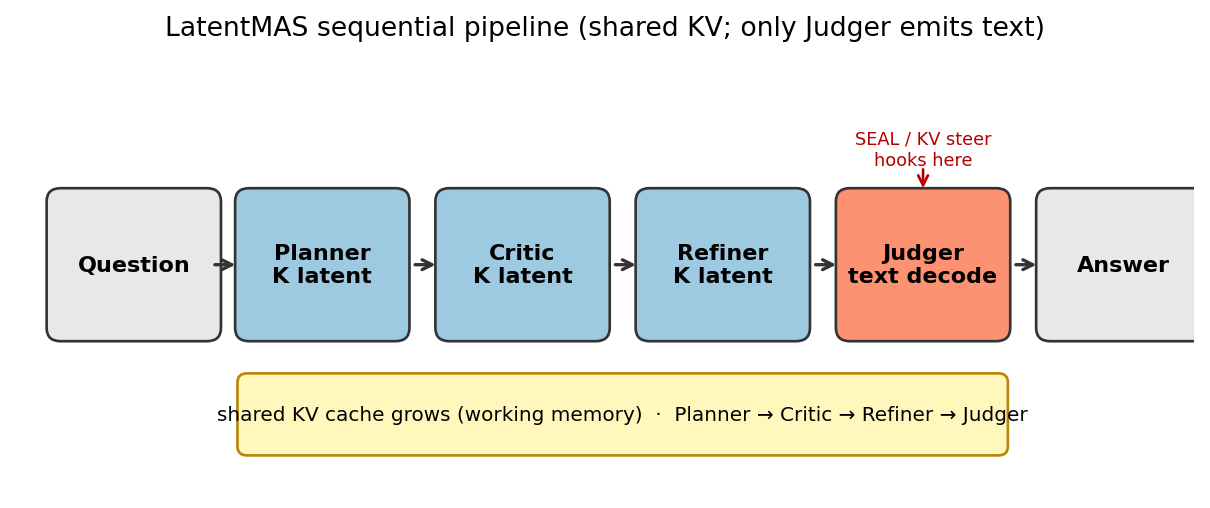
\includegraphics[width=0.95\textwidth]{arch_latentmas.png}
    \end{center}
    \vspace{-0.15cm}
    \begin{itemize}\footnotesize
        \item Sequential topology used throughout: Planner $\rightarrow$ Critic $\rightarrow$ Refiner $\rightarrow$ Judger.
        \item Default $K{=}40$ latent forwards per upstream agent; total latent compute $\approx 3(K{+}1)$.
        \item Output-token metric $=$ Judger generations to EOS (the only place tokens exist to shrink).
    \end{itemize}
\end{frame}

%=============================================================================
\begin{frame}{Technical Background: Activation Steering / SEAL}
    \textbf{Paper:} Chen et al., \emph{SEAL} (arXiv:2504.07986) --- training-free reasoning calibration.
    \begin{itemize}
        \item Long CoT mixes \textbf{execution} (carry solution forward), \textbf{reflection} (``wait / check''), \textbf{transition} (``alternatively''). Excess reflection/transition $\Leftrightarrow$ overthinking.
        \item Thought types are \textbf{linearly separable} in deep residual streams.
        \item Offline, from $\sim$50 GSM8K-train traces at layer $L{=}28$:
        \[
          v = \mu_{\text{exec}} - \mu_{\text{refl}\,\cup\,\text{trans}}
          \quad (\text{raw }\lVert v\rVert \approx 52.7)
        \]
        \item Online hook on decoder layer $L$: $h_{:,-1,:} \mathrel{+}= \alpha\, \hat{v}$. \\
        $\alpha > 0$ suppresses reflection $\Rightarrow$ shorter decode; $\alpha{=}0$ $=$ plain LatentMAS.
    \end{itemize}
\end{frame}

%=============================================================================
\begin{frame}{SEAL Mechanically}
    \begin{center}
        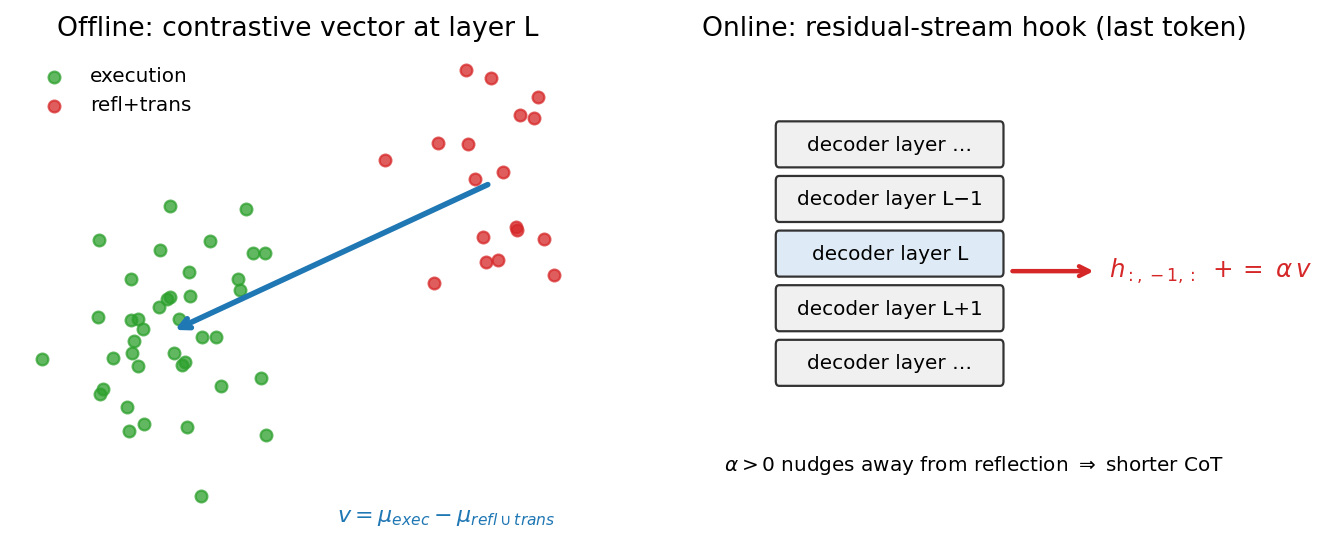
\includegraphics[width=0.98\textwidth]{seal_mechanism.png}
    \end{center}
    \vspace{-0.1cm}
    \begin{itemize}\footnotesize
        \item Hook registered once (\texttt{SealSteerer}); enabled/disabled \textbf{per agent role} (\texttt{--seal\_agents}).
        \item Applied every Judger forward during \texttt{generate\_text\_batch}; negligible latency vs.\ decode.
        \item Same residual site later reused for \textbf{native} vectors and trainable CES $v$.
    \end{itemize}
\end{frame}

%=============================================================================
\begin{frame}{Why Steer the Judger First?}
    \textbf{Architectural consequence, not a modeling preference}
    \begin{itemize}
        \item Planner / Critic / Refiner run a \textbf{fixed} $K$-step latent loop --- no variable-length text.
        \item Every output token the system emits comes from the Judger's AR decode.
        \item Therefore a length/token objective can only bite the Judger; upstream SEAL can at best change \emph{quality} of the KV the Judger reads.
        \item Early pilot: steering latent agents alone $\Rightarrow$ no token change (by construction) and no clear accuracy win.
    \end{itemize}
    \vspace{0.2cm}
    \begin{center}\textit{Research question becomes: does Judger SEAL cut tokens at matched accuracy?}\\
    \textit{Then: can upstream / handoff / smaller-$K$ steering still help?}\end{center}
\end{frame}

%=============================================================================
\begin{frame}{Fork Fidelity (before any intervention)}
    \textbf{Two independent proofs on} \texttt{Gen-Verse/LatentMAS@9a9e4d3}
    \begin{itemize}
        \item \textbf{Byte-for-byte:} all 24 upstream file SHAs match (0 mismatches).
        \item \textbf{Behavioral:} Qwen3-14B accuracy within noise of the paper.
    \end{itemize}
    \vspace{0.15cm}
    \begin{table}
        \centering\small
        \begin{tabular}{lcc}
            \toprule
            Task & Our fork & Paper \\
            \midrule
            GSM8K & 92.7\% & 95.2\% \\
            ARC-Challenge & 94.7\% & 95.6\% \\
            MedQA & 79.3\% & 80.7\% \\
            \bottomrule
        \end{tabular}
    \end{table}
    \vspace{0.1cm}
    \begin{center}\footnotesize Subset / single seed / stochastic decode vs.\ paper's 3-seed full-set means.\end{center}
\end{frame}

%=============================================================================
\begin{frame}{Protocol (SEAL A/B)}
    \begin{table}
        \centering\small
        \begin{tabular}{ll}
            \toprule
            Parameter & Value \\
            \midrule
            Model & Qwen/Qwen3-14B (40 layers, $d{=}5120$) \\
            Topology & sequential; $K{=}40$ upstream \\
            Datasets & GSM8K, ARC-C, MedQA \\
            $n$ / seed & 120 / 100; seed 42 \\
            Sampling & $T{=}0.6$, top-$p{=}0.95$ \\
            SEAL layer / vector & 28; GSM8K-train MoD \\
            Metric & accuracy + mean Judger tokens \\
            Backend & HF, 1$\times$ H200 \\
            \bottomrule
        \end{tabular}
    \end{table}
\end{frame}

%=============================================================================
\section{Part I: Judger SEAL}
\begin{frame}{Main Result: Judger Dose--Response}
    \begin{center}
        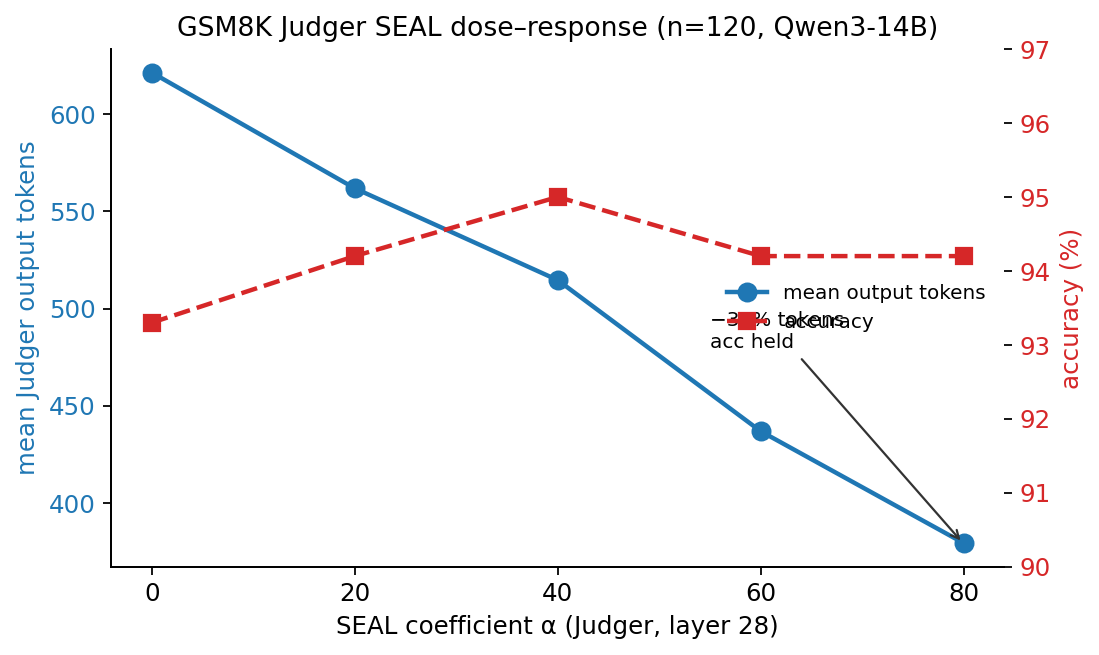
\includegraphics[width=0.88\textwidth]{dose_response_gsm8k.png}
    \end{center}
    \vspace{-0.15cm}
    \begin{itemize}\footnotesize
        \item Monotonic token cut: $-$17\% (coef 40) $\rightarrow$ $-$39\% (coef 80); accuracy held or \emph{improved}.
        \item $\sim$2$\times$ faster Judger decode at coef 80 --- real over-reasoning ($\sim$620 tok baseline).
    \end{itemize}
\end{frame}

%=============================================================================
\begin{frame}{Numbers Behind the Curve}
    \begin{table}
        \centering\small
        \begin{tabular}{cccc}
            \toprule
            coef $\alpha$ & Accuracy & Mean tokens & $\Delta$ tokens \\
            \midrule
            0 (control) & 93.3\% & 621 & --- \\
            40 & \textbf{95.0\%} & 515 & $-$17\% \\
            60 & 94.2\% & 437 & $-$30\% \\
            80 & 94.2\% & 379 & \textbf{$-$39\%} \\
            \bottomrule
        \end{tabular}
    \end{table}
    \vspace{0.25cm}
    \begin{block}{Interpretation}
        SEAL's execution$-$reflection axis is a \textbf{verbosity / overthinking} direction in Judger residual space. Positive $\alpha$ shortens CoT without collapsing answer quality on GSM8K.
    \end{block}
\end{frame}

%=============================================================================
\begin{frame}{Cross-Task Transfer}
    \begin{center}
        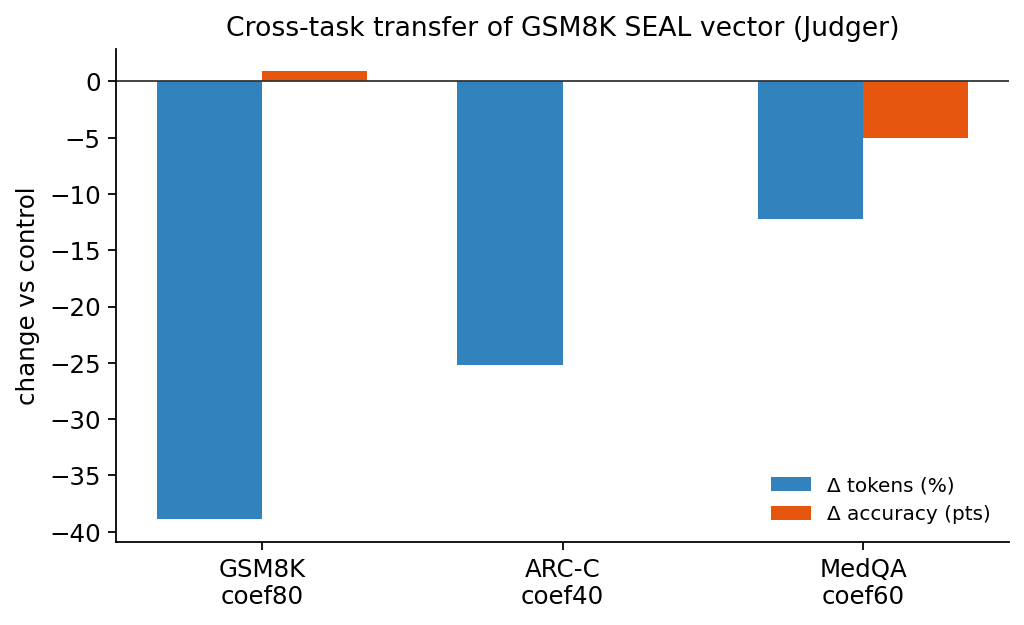
\includegraphics[width=0.82\textwidth]{transfer_bars.png}
    \end{center}
    \vspace{-0.1cm}
    \begin{itemize}\footnotesize
        \item ARC-C: \textbf{$-$25\% tokens at identical accuracy} (coef 40) --- clean transfer.
        \item MedQA: coef-sensitive (early coef60: $-$12\% tok / $-$5 pts; later held-out coef80: $+2$ pts / $-$26\%).
        \item Same GSM8K vector, no re-extraction --- supports SEAL's claim of a general overthinking axis.
    \end{itemize}
\end{frame}

%=============================================================================
\section{Part II: Who Can We Steer?}
\begin{frame}{Per-Agent Ablation: Only Judger Moves Tokens}
    \begin{center}
        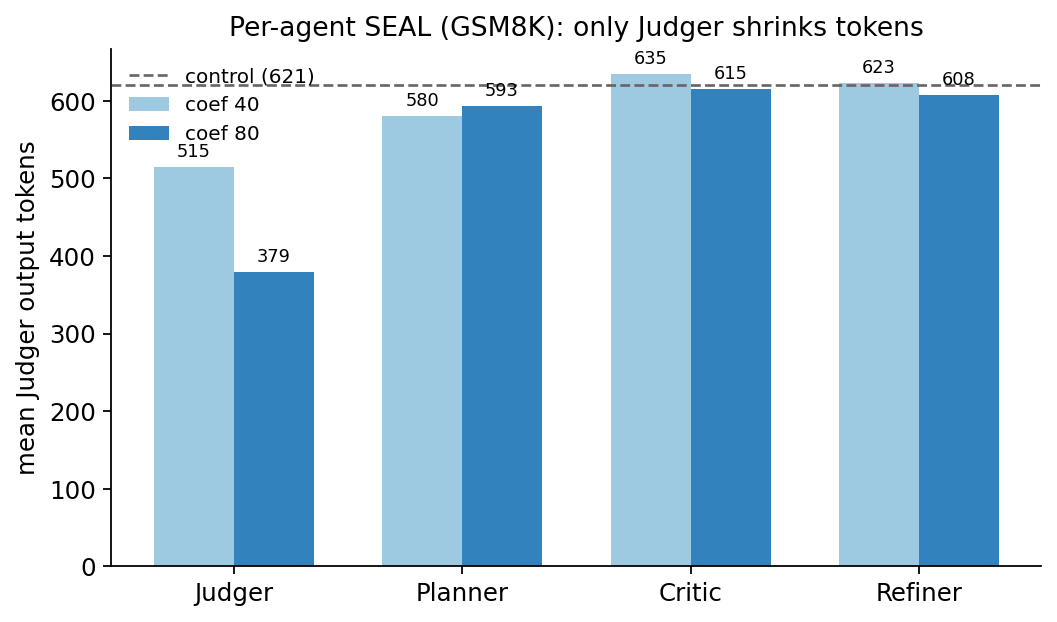
\includegraphics[width=0.85\textwidth]{per_agent_tokens_gsm8k.png}
    \end{center}
    \vspace{-0.1cm}
    \begin{itemize}\footnotesize
        \item Same GSM8K SEAL vector, one role enabled at a time.
        \item Steering all agents $\approx$ Judger-only --- upstream contribution to length is $\approx 0$.
    \end{itemize}
\end{frame}

%=============================================================================
\begin{frame}{Why? Thought Mix Is Uniform}
    \begin{center}
        
\includegraphics[width=0.82\textwidth]{agent_thoughts_gsm8k.png}
    \end{center}
    \vspace{-0.1cm}
    \begin{itemize}\footnotesize
        \item $\sim$88\% execution for \emph{every} role --- Judger is not ``more reflective.''
        \item Effect is \textbf{structural}: only Judger has a variable-length text channel.
        \item Caveat: isolation proxy (roles prompted alone in text).
    \end{itemize}
\end{frame}

%=============================================================================
\begin{frame}{Technical: Native Correctness-Contrastive Vectors}
    \textbf{New objective for latent agents (quality, not length)}
    \begin{itemize}
        \item Capture each agent's \textbf{in-pipeline} layer-28 residual (conditioned on upstream KV), mean-pool per run.
        \item Label by \textbf{final answer correctness}; build
        \[
          v_{\text{agent}} = \mu(h \mid \text{correct}) - \mu(h \mid \text{incorrect}).
        \]
        \item Apply during that agent's forwards; evaluate end-to-end accuracy + Judger tokens.
        \item Mechanistic check: 5-fold linear probe AUC of $h$ $\rightarrow$ correctness (how early is the outcome decided?).
    \end{itemize}
\end{frame}

%=============================================================================
\begin{frame}{Mechanism: Correctness Is Decided Late}
    \begin{center}
        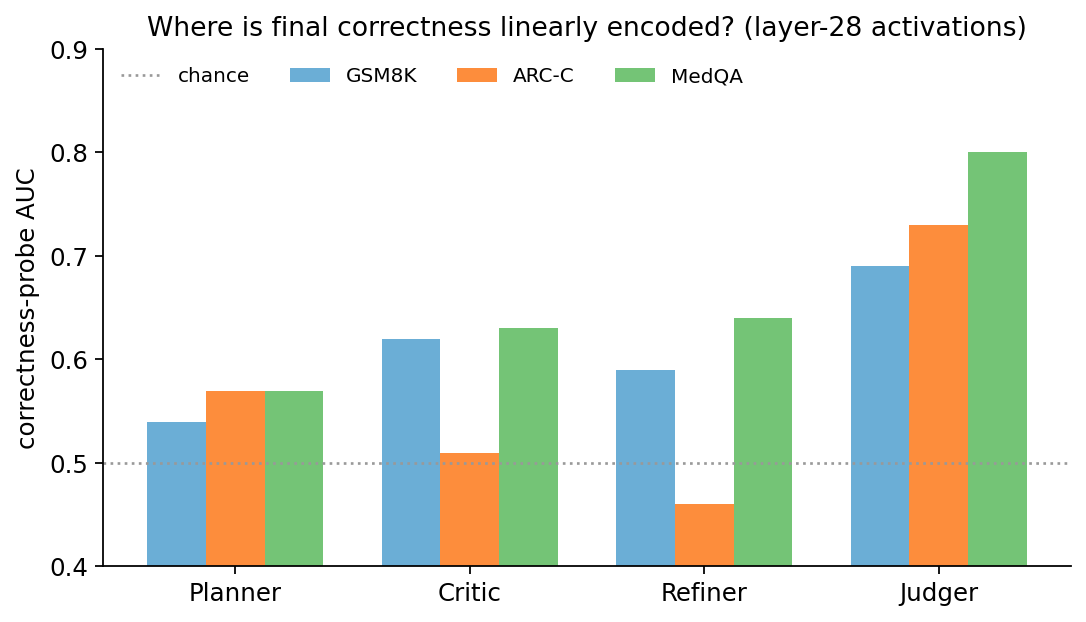
\includegraphics[width=0.88\textwidth]{probe_auc_all.png}
    \end{center}
    \vspace{-0.1cm}
    \begin{itemize}\footnotesize
        \item Upstream AUC 0.46--0.64 (near chance); Judger 0.69--0.80.
        \item Wrong answers over-generate \textbf{+70--82\%} tokens --- length coupled to failure \emph{at Judger}.
        \item Predicts: steering fixed-runtime upstream agents cannot smooth a late decision.
    \end{itemize}
\end{frame}

%=============================================================================
\begin{frame}{Native Sweep: Honest Negative}
    \begin{center}
        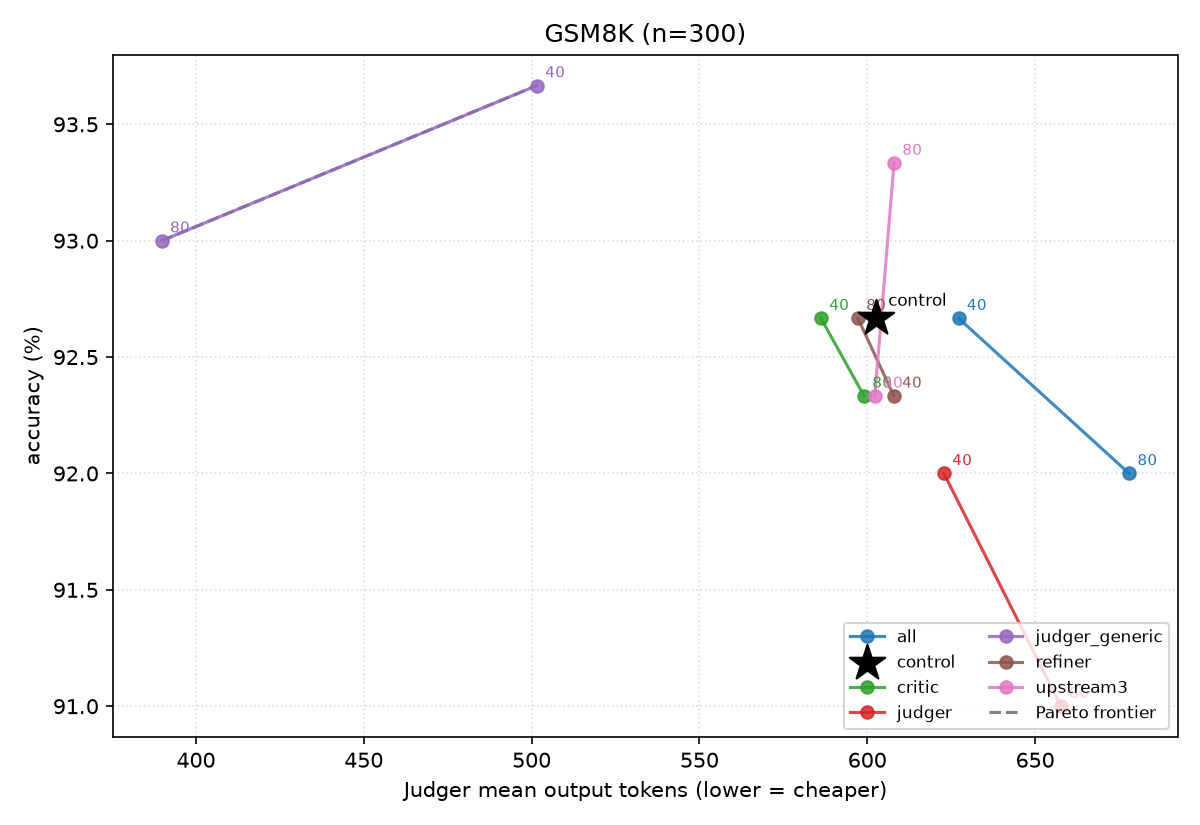
\includegraphics[width=0.78\textwidth]{pareto_gsm8k.png}
    \end{center}
    \vspace{-0.15cm}
    \begin{itemize}\footnotesize
        \item Purple \textbf{judger\_generic} dominates up-and-left; every native/upstream config hugs control.
        \item Native Judger vector is \emph{worse} than generic SEAL --- toward-correct $\neq$ shorter.
        \item Same story on ARC / MedQA Pareto plots (assets).
    \end{itemize}
\end{frame}

%=============================================================================
\begin{frame}{Native vs Generic (GSM8K test, $n{=}300$)}
    \begin{table}
        \centering\footnotesize
        \begin{tabular}{lccc}
            \toprule
            Steering & coef & Acc & Tokens \\
            \midrule
            control & 0 & 92.7\% & 602 \\
            Critic (native) & 40 & 92.7\% & 586 \\
            Upstream-3 (native) & 80 & 93.3\% & 608 \\
            Judger (native) & 80 & 91.0\% & 658 \\
            \textbf{Judger (generic SEAL)} & 80 & 93.0\% & \textbf{390 ($-$35\%)} \\
            \bottomrule
        \end{tabular}
    \end{table}
    \vspace{0.2cm}
    \begin{block}{Verdict}
        For token efficiency in sequential latent MAS, \textbf{Judger-only SEAL is sufficient and dominant}. Isolation-proxy Phase-C critic gains do not survive native end-to-end eval.
    \end{block}
\end{frame}

%=============================================================================
\section{Part III: KV Cache Steering}
\begin{frame}{Technical: KV Cache Steering}
    \textbf{Paper:} \emph{KV Cache Steering for Controlling Frozen LLMs} (arXiv:2507.08799).
    \begin{itemize}
        \item One-shot edit of past keys/values, then normal decode --- \emph{no} per-step residual hook:
        \[
          K \mathrel{+}= c_k S_k,\qquad V \mathrel{+}= c_v S_v
        \]
        (we use value-only, $c_k{=}0$).
        \item Direction $S$ from 200 GSM8K-train contrastive pairs: CoT-rich vs answer-only ICL.
        \item Surfaces in LatentMAS:
        \begin{itemize}
            \item \texttt{handoff\_last} / \texttt{handoff\_all} --- latent KV the Judger inherits;
            \item \texttt{judger\_token} --- Judger's own last prompt token (paper's intended surface).
        \end{itemize}
    \end{itemize}
\end{frame}

%=============================================================================
\begin{frame}{KV Results: Handoff Fails; Judger Token Wins}
    \begin{center}
        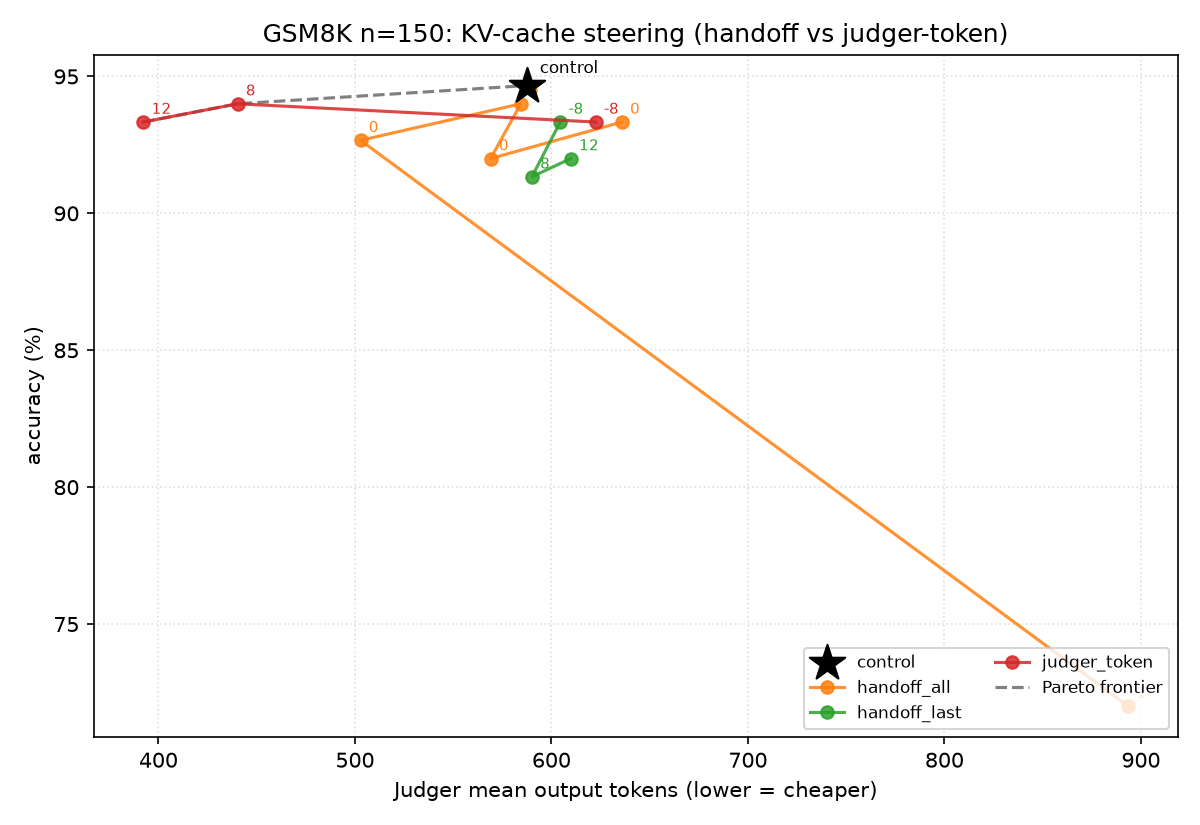
\includegraphics[width=0.78\textwidth]{kv_gsm8k.png}
    \end{center}
    \vspace{-0.1cm}
    \begin{itemize}\footnotesize
        \item \texttt{handoff\_all} $c_v{=}1$: accuracy collapses 94.7\%$\rightarrow$72\% (attention saturation --- full shift of Judger attention output).
        \item \texttt{judger\_token} $c_v{=}{+}12$: \textbf{$-$33\% tokens}, accuracy within noise --- third independent Judger-side win.
    \end{itemize}
\end{frame}

%=============================================================================
\section{Part IV: K-Budget CES}
\begin{frame}{Technical: K-Budget + CES Hypothesis}
    \textbf{Option 1 claim (now stopped at Gate~1)}
    \begin{itemize}
        \item Reduce per-agent latent budget $K_{\text{small}} < K_{\text{full}}$ to save compute.
        \item Learn a residual steering vector $v$ (CES / ASC-style) applied during upstream \textbf{latent steps only}, so small-$K$ recovers full-$K$ accuracy.
        \item Primary compute metric: \textbf{wall-clock latency} (not raw forward count --- KV length grows, forwards unequal cost).
        \item Gate~1 must show: credible accuracy gap \emph{and} $\geq$15\% latency savings at $K_{\text{small}}$.
        \item Gate~2 (grad smoke on Qwen3-4B) already passed; do \textbf{not} scale training without Gate~1.
    \end{itemize}
\end{frame}

%=============================================================================
\begin{frame}{Gate 1: MedQA $K$-Curve}
    \begin{center}
        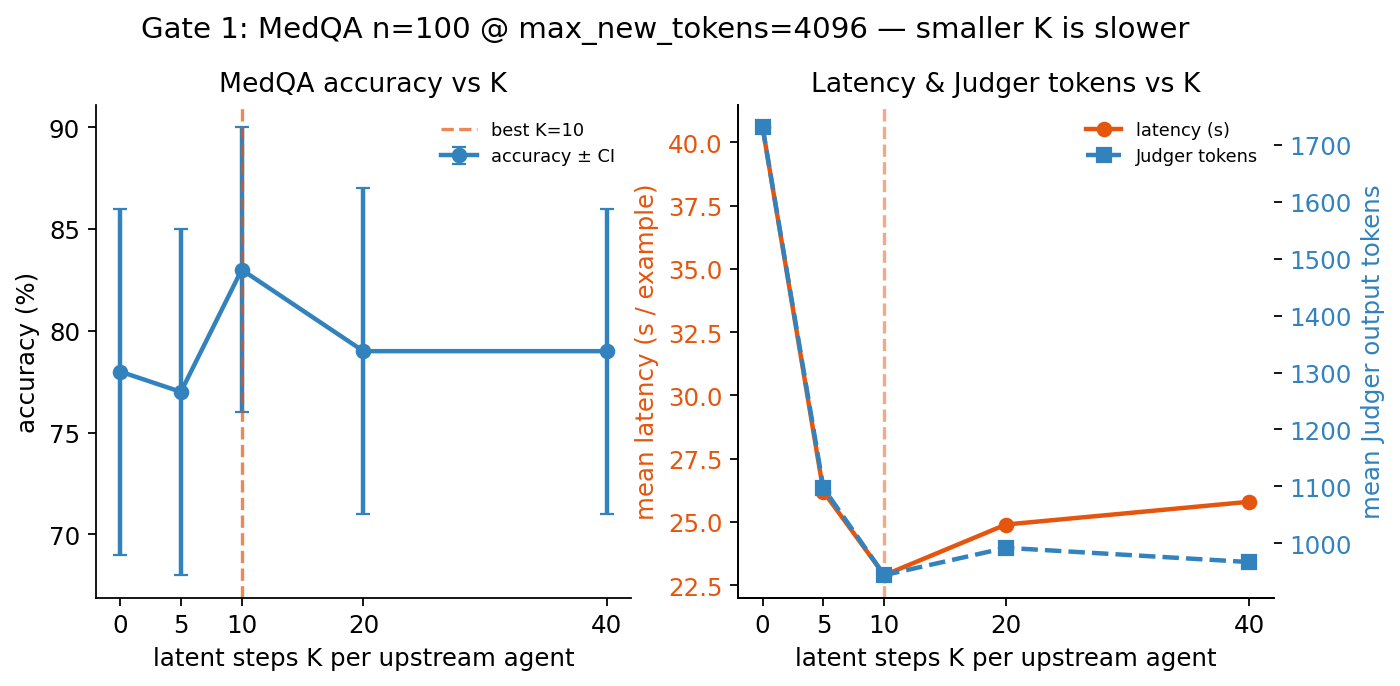
\includegraphics[width=0.95\textwidth]{gate1_medqa_kcurve.png}
    \end{center}
    \vspace{-0.1cm}
    \begin{itemize}\footnotesize
        \item Best accuracy \emph{and} best latency at \textbf{$K{=}10$}, not $K{=}40$.
        \item Cutting $K$ increases Judger tokens $\Rightarrow$ system gets \textbf{slower}.
    \end{itemize}
\end{frame}

%=============================================================================
\begin{frame}{Gate 1 Probe: AIME 2024 @ 8192}
    \begin{center}
        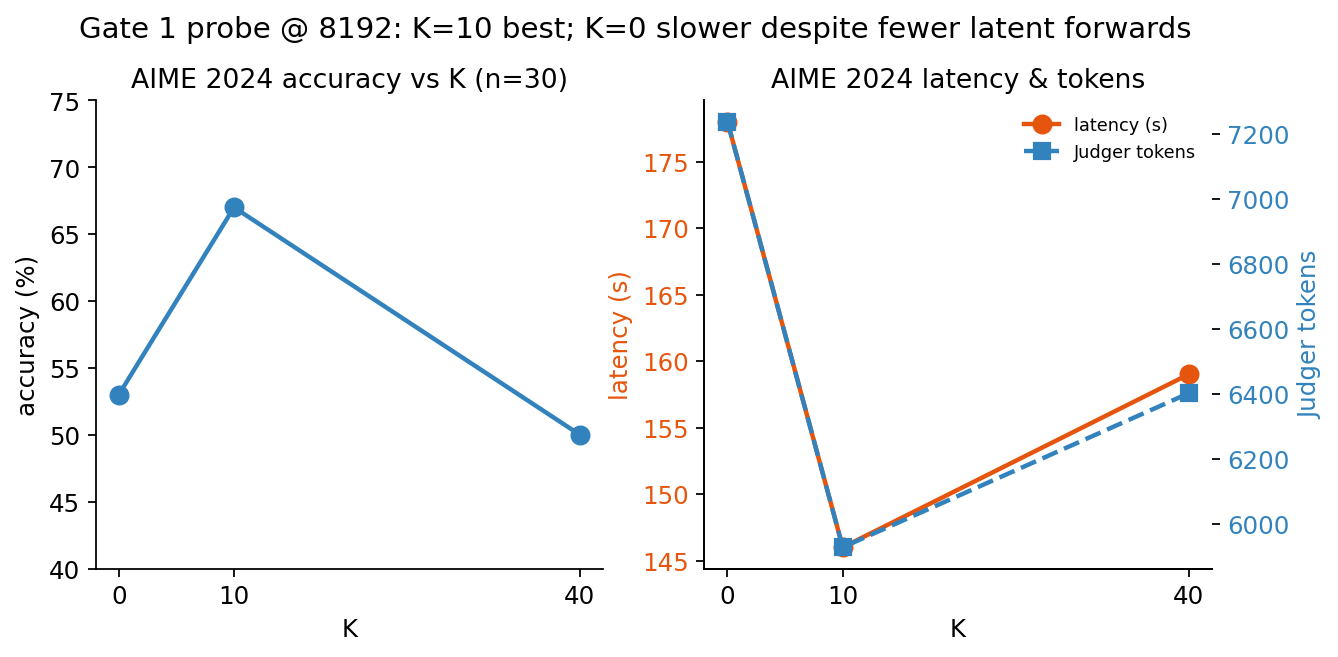
\includegraphics[width=0.92\textwidth]{gate1_aime_kcurve.png}
    \end{center}
    \vspace{-0.1cm}
    \begin{itemize}\footnotesize
        \item Credible paired gap $K{=}10 - K{=}0 \approx +13$ pts --- but $K{=}0$ is $\sim$21\% \emph{slower}.
        \item Extra latent steps often \textbf{shorten} Judger CoT enough to more than pay for themselves.
    \end{itemize}
\end{frame}

%=============================================================================
\begin{frame}{Gate 1 Verdict: STOP K-Budget CES}
    \begin{table}
        \centering\small
        \begin{tabular}{lcc}
            \toprule
            Criterion & MedQA & AIME@8192 \\
            \midrule
            Credible acc($K_{\text{full}}\!>\!K_{\text{small}}$) & Weak / wrong dir. & Yes ($10$ vs $0$) \\
            $\geq$15\% wall-clock cut at $K_{\text{small}}$ & \textbf{No} & \textbf{No} \\
            Proceed to CES train & \textbf{No} & \textbf{No} \\
            \bottomrule
        \end{tabular}
    \end{table}
    \vspace{0.25cm}
    \begin{block}{Root cause}
        Wall-clock is \textbf{Judger-token--dominated}. Smaller $K$ $\Rightarrow$ longer Judger CoT $\Rightarrow$ slower system. \\
        Do \textbf{not} start CES pair mining for K-budget recovery.
    \end{block}
\end{frame}

%=============================================================================
\section{Synthesis}
\begin{frame}{Where Reasoning Lives}
    \begin{center}
        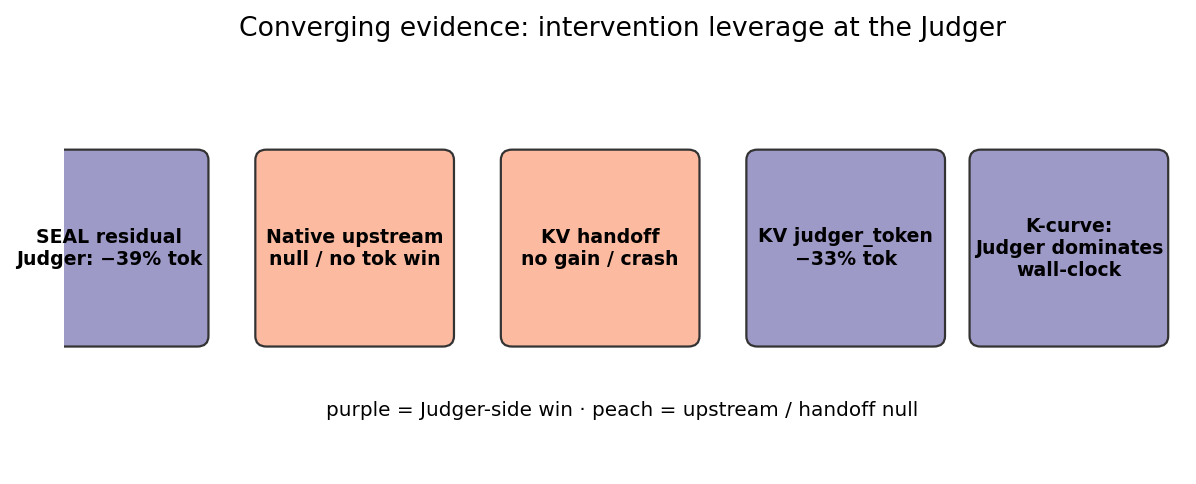
\includegraphics[width=0.95\textwidth]{synthesis_localization.png}
    \end{center}
    \vspace{-0.1cm}
    \begin{center}
        Four independent lines: residual SEAL, native contrastive, KV surfaces, and the $K$-curve \\
        all localize effective intervention at the \textbf{Judger}.
    \end{center}
\end{frame}

%=============================================================================
\begin{frame}{What's the Contribution}
    \begin{enumerate}
        \item \textbf{Analysis / localization (strongest):} where reasoning is decided in latent MAS, and why upstream steering fails (probes + three methods + $K$-curve).
        \item \textbf{Method:} Judger residual / cache steering for token-efficient latent MAS ($-$25 to $-$39\% tokens, accuracy held, transfers).
    \end{enumerate}
    \vspace{0.35cm}
    \begin{block}{Preferred pivot after Gate~1}
        Double down on \textbf{Judger-side} ASC / SEAL-style CoT compression --- not K-budget recovery.
    \end{block}
\end{frame}

%=============================================================================
\begin{frame}{Limitations}
    \begin{enumerate}
        \item \textbf{Power:} $n{=}100$--$300$ (AIME $n{=}30$), mostly single seed.
        \item \textbf{Coverage:} one layer (28), one backbone (Qwen3-14B).
        \item \textbf{Task sensitivity:} MedQA coef-dependent.
        \item \textbf{Proxies:} isolation thought-types; capture mean-pools; class imbalance on easy tasks.
        \item \textbf{Modality:} SEAL/KV directions extracted from text CoT, applied under latent conditioning.
    \end{enumerate}
\end{frame}

%=============================================================================
\begin{frame}{Next Steps}
    \begin{itemize}
        \item $n{\approx}500$, 3 seeds, full Judger accuracy--token Pareto.
        \item Gentler coef / layer sweep for MedQA Judger steering.
        \item Optional method paper: Judger ASC / learned compression.
        \item If upstream again: hierarchical topology or process objectives --- \textbf{not} K-budget wall-clock recovery.
        \item Position against cache-steering / RepE baselines (partially done).
    \end{itemize}
\end{frame}

%=============================================================================
\begin{frame}{Conclusion}
    \begin{center}
        \Large \textbf{Core Message}\\[0.45cm]
        \normalsize
        SEAL on the LatentMAS \textbf{Judger} cuts output tokens \textbf{$\sim$25--39\% with accuracy retained}, and the vector \textbf{transfers}.\\[0.35cm]
        The gain is \textbf{localized to the text-emitting agent}. Upstream residual, native, and KV handoff steering do not move the frontier; the $K$-curve shows why wall-clock is Judger-dominated.\\[0.35cm]
        \textbf{Stop} K-budget CES. Pivot to Judger-side token compression --- where steering actually works.
    \end{center}
\end{frame}

\end{document}
